\chapter{Oracle Aplication Express}

\section{Pengenalan Oracle APEX}
Oracle Aplication Express\cite{OracleApex}. Adalah sebuah wadah dan sarana untuk membuat aplikasi yang menggunakan database Oracle Itu sendiri, pada akademi oracle ini bertujuan untuk memajukan ilmu komputer  secara global untuk  mendorong pengetahuan, inovasi, pengembangan keterampilan dan keragaman di bidang teknologi. Disini saya diajarkan membuat Request Workspace, Create Workspace, Membuat Spreadsheet Pertama.

\section{Tahapan Membuat Aplikasi Oracle Apex}
Langkah pertama yang dilakukan adalah membuka website resmi dari Oracle Apex yaitu https://apex.oracle.com , disini kita akan mendapatkan akses untuk memasuki Oracle Apllication Express. Pastikan email anda sudah terdaftar dan sudah terverifikasi dan bisa digunakan untuk membuat Workspace. Berikut tahapan pembuatan Aplikasi pada Oracle Appliction Express :

\begin{enumerate}
\item[1]Pergi ke website resmi Oracle.

\begin{figure}[!htbp]
    \begin{center}
    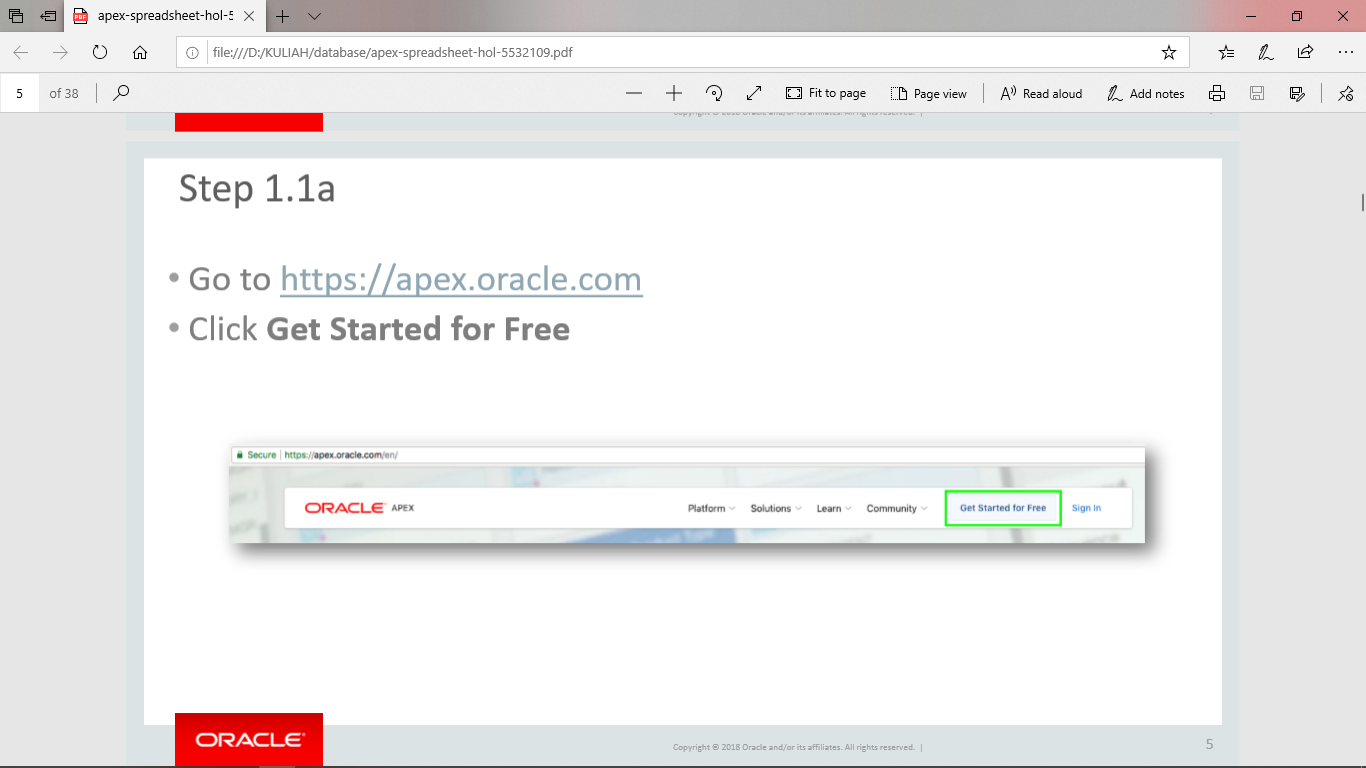
\includegraphics[scale=0.2]{figures/pic(1).png}
    \caption{\textit{Get Start For Free.}}
    \end{center}   
    \end{figure}
    
\begin{figure}[!htbp]
\item[2]Klik Request a Free Worksace.

    \begin{center}
    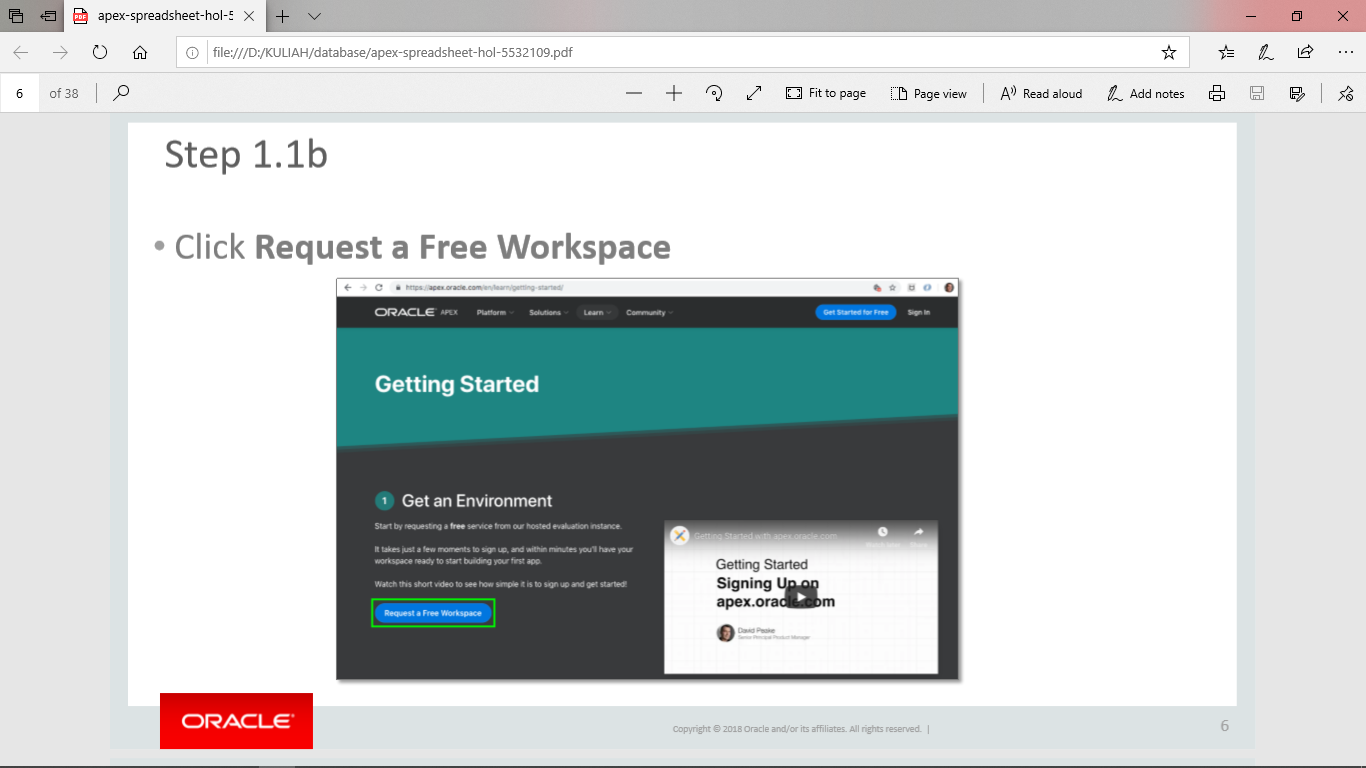
\includegraphics[scale=0.2]{figures/pic(2).png}
    \caption{\textit{Request A Free Workspace.}}
    \end{center}

\item[3]Isikan data diri anda seperti nama,email,dan workspace.

   
        
\item[4]Centang apakah anda pernah melakukan hal tersebut lalu next.  



\item[5]Isikan pada kolom tersebut bebas, mengapa anda ingin menggunakan layanan ini ?, lalu klik next.

    


\item[6] Centang Accept, lalu klik next.

  
\item[7] Tahapan terakhir untuk mengkonfirmasi apakah ini anda, lalu klik next.

   
\item[8] Finish, lalu lihat email anda.

    \begin{center}
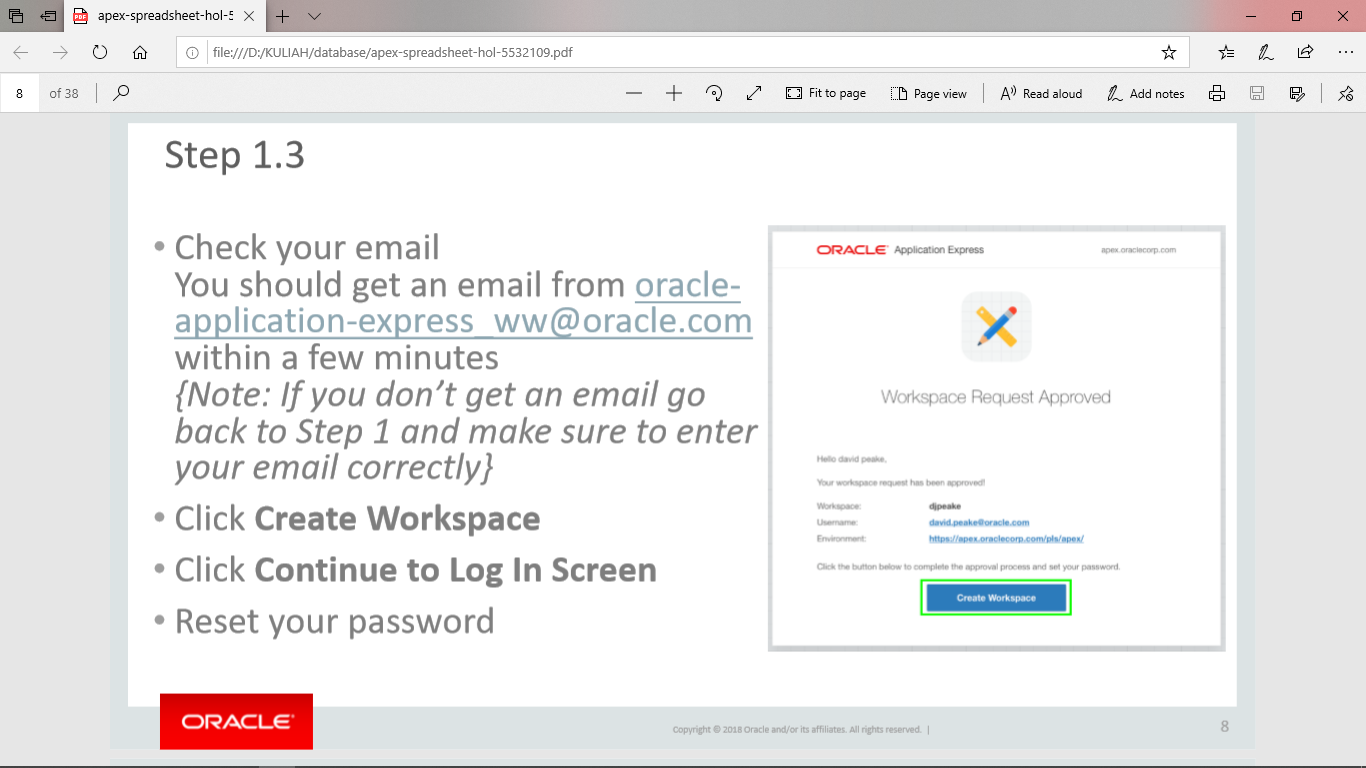
\includegraphics[scale=0.2]{figures/pic(3).png}
    \caption{\textit{Sukses Cek Email.}}
        \end{center}
\label{gambar}
\end{figure}

\begin{figure}
\item[9] Selamat Workspace anda telah di Acc lalu klik continue.

    \begin{center}
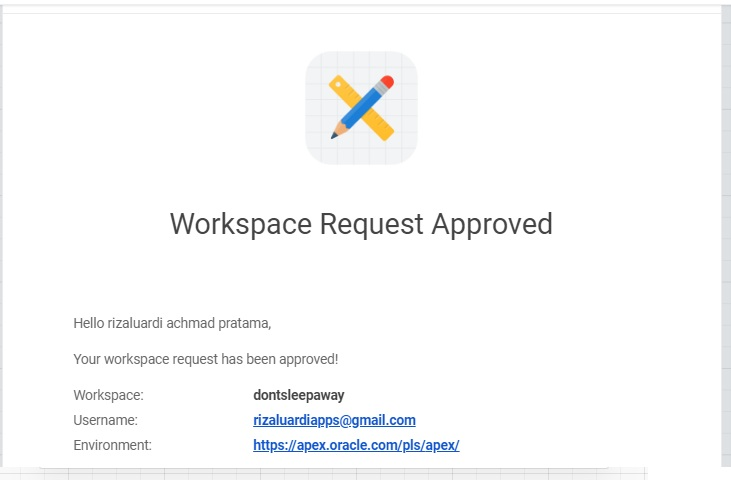
\includegraphics[scale=0.5]{figures/req7.jpg}
    \caption{\textit{Email Acc.}}
        \end{center}
\label{gambar}
\end{figure}

\begin{figure}
\item[10] Workspace kamu telah dibut lalu lanjutkan klik sign in.

    \begin{center}
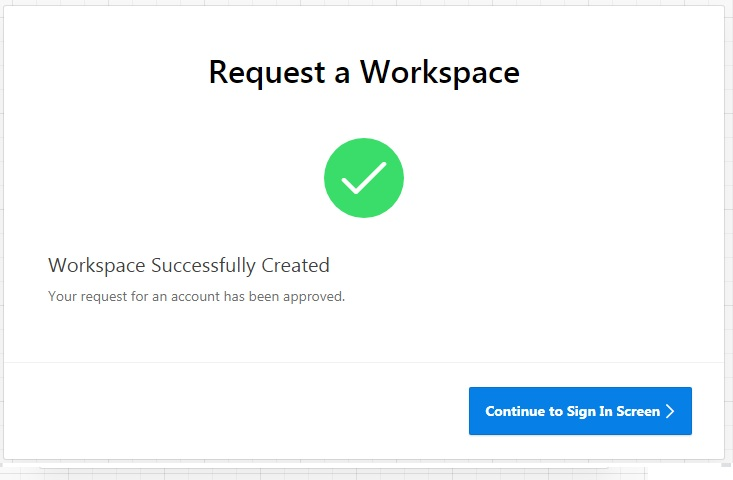
\includegraphics[scale=0.5]{figures/req8.jpg}
    \caption{\textit{Sukses Cek Email.}}
        \end{center}
\label{gambar}
\end{figure}

\begin{figure}
\item[11] Sign in akun anda yang baru saja di buat lalu masuk ke app builder lalu buat app baru.

    \begin{center}
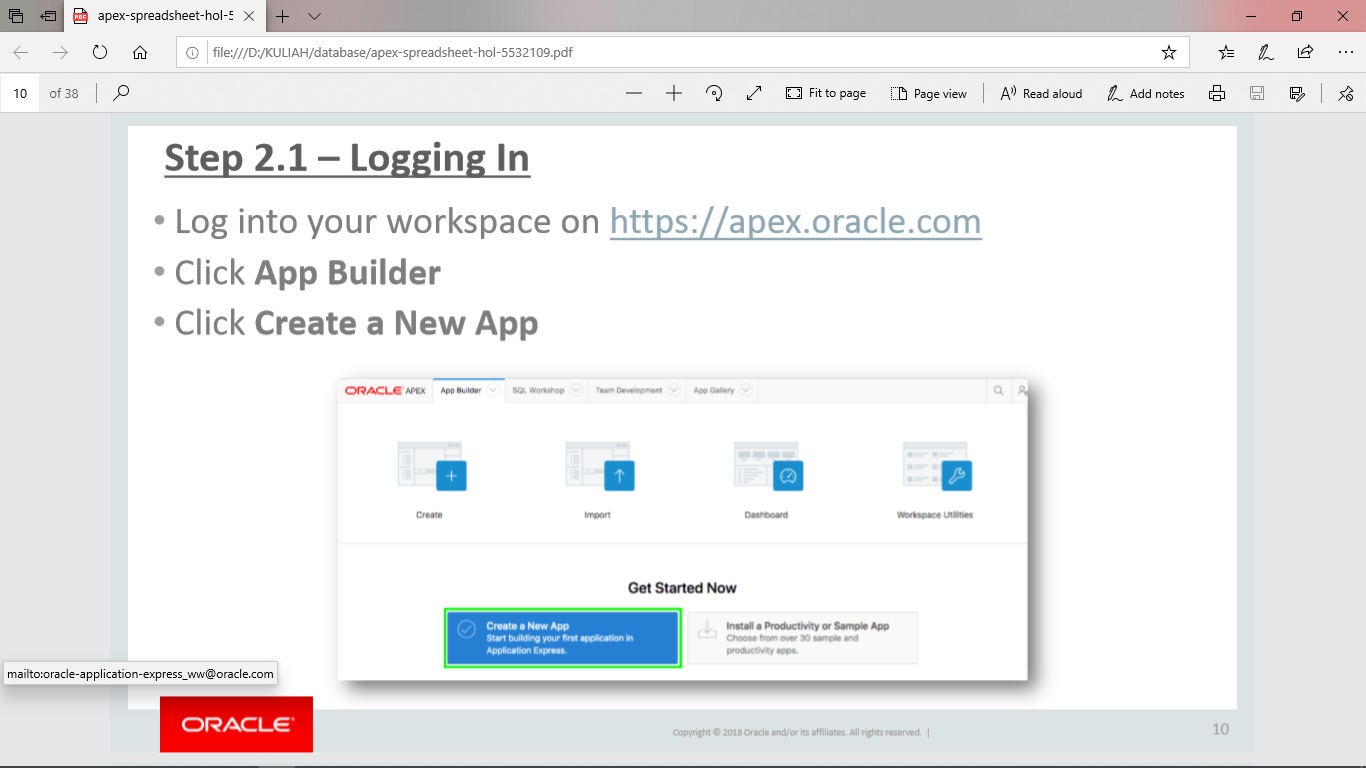
\includegraphics[scale=0.3]{figures/pic(4).png}
    \caption{\textit{Sign in oracle.}}
        \end{center}
\label{gambar}
\end{figure}

\begin{figure}
\item[12] Lalu pilih from a file

    \begin{center}
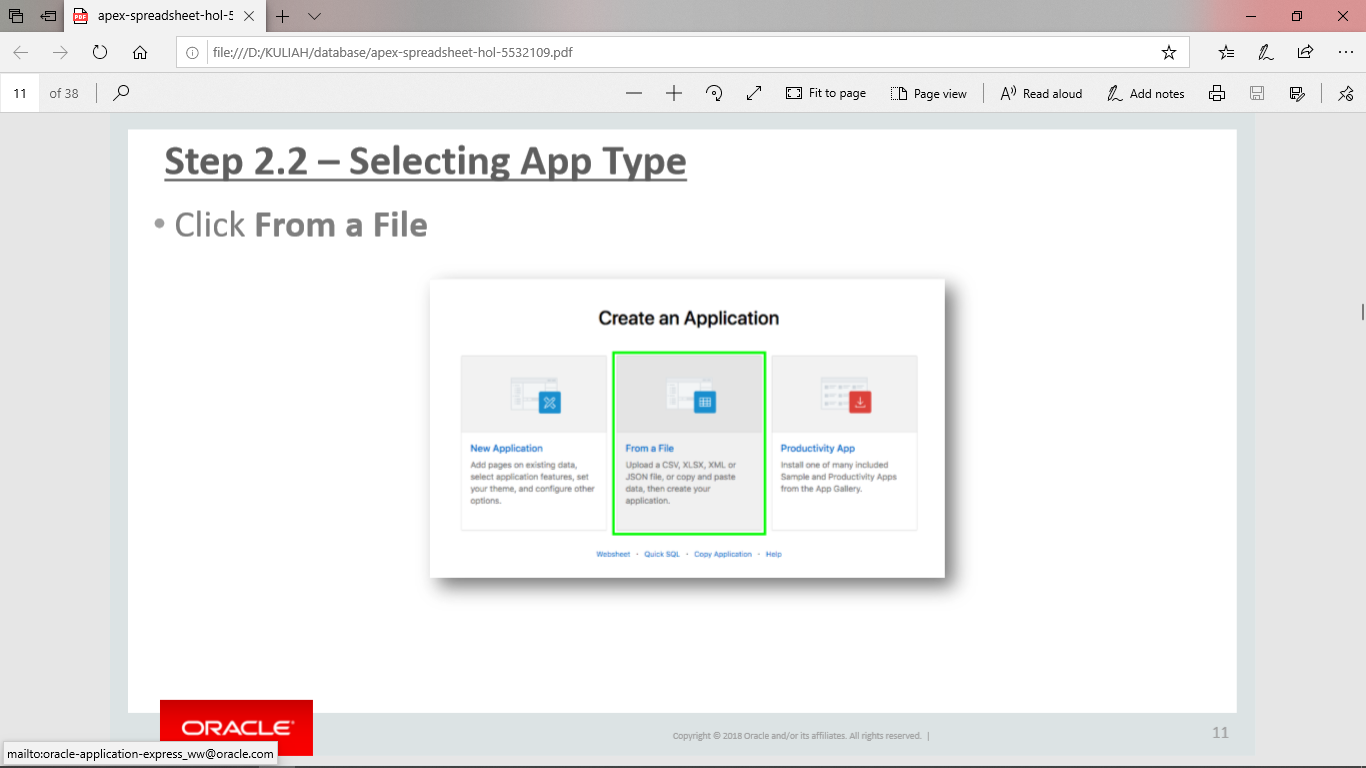
\includegraphics[scale=0.3]{figures/pic(5).png}
    \caption{\textit{select app type.}}
        \end{center}
\label{gambar}
\end{figure}

\begin{figure}
\item[13] Klik Copy and Paste.

    \begin{center}
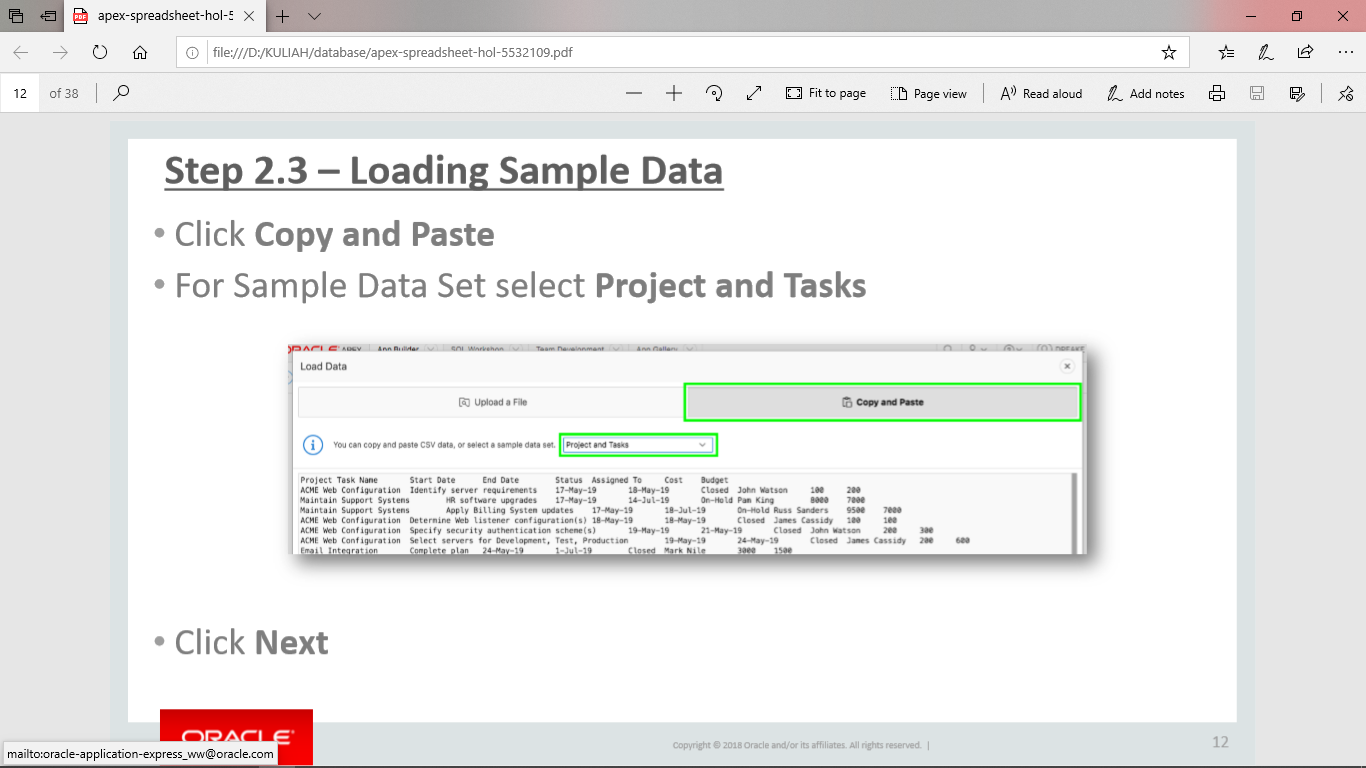
\includegraphics[scale=0.3]{figures/pic(6).png}
    \caption{\textit{Copy and Paste.}}
        \end{center}
\label{gambar}
\end{figure}

\begin{figure}
\item[14] Beri nama table (spreadsheet) dan klik load data supaya data dimuat oleh sistem.

    \begin{center}
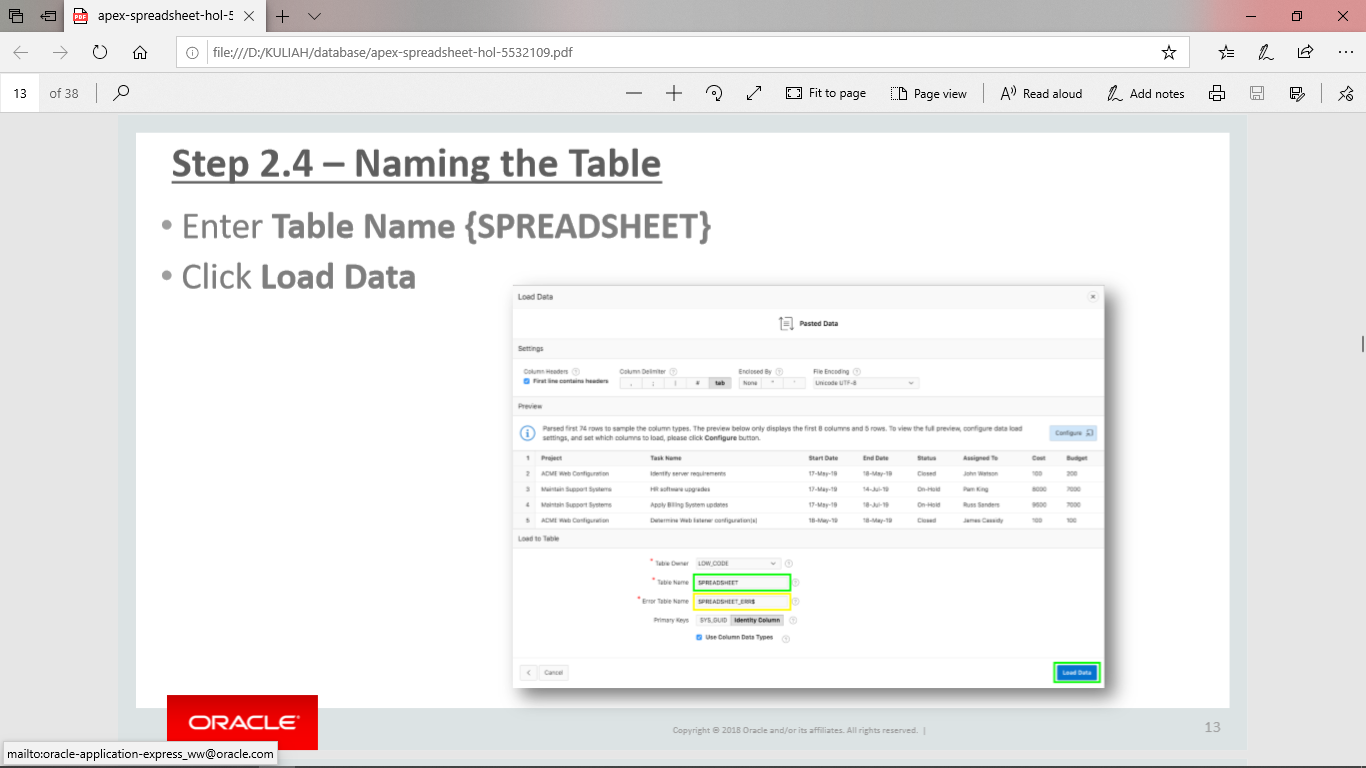
\includegraphics[scale=0.3]{figures/pic(7).png}
    \caption{\textit{penamaan tabel dan memuat data.}}
        \end{center}
\label{gambar}
\end{figure}

\begin{figure}
\item[15] Setelah Sudah me-Load data, tampilan selanjutnya akan seperti berikut.

    \begin{center}
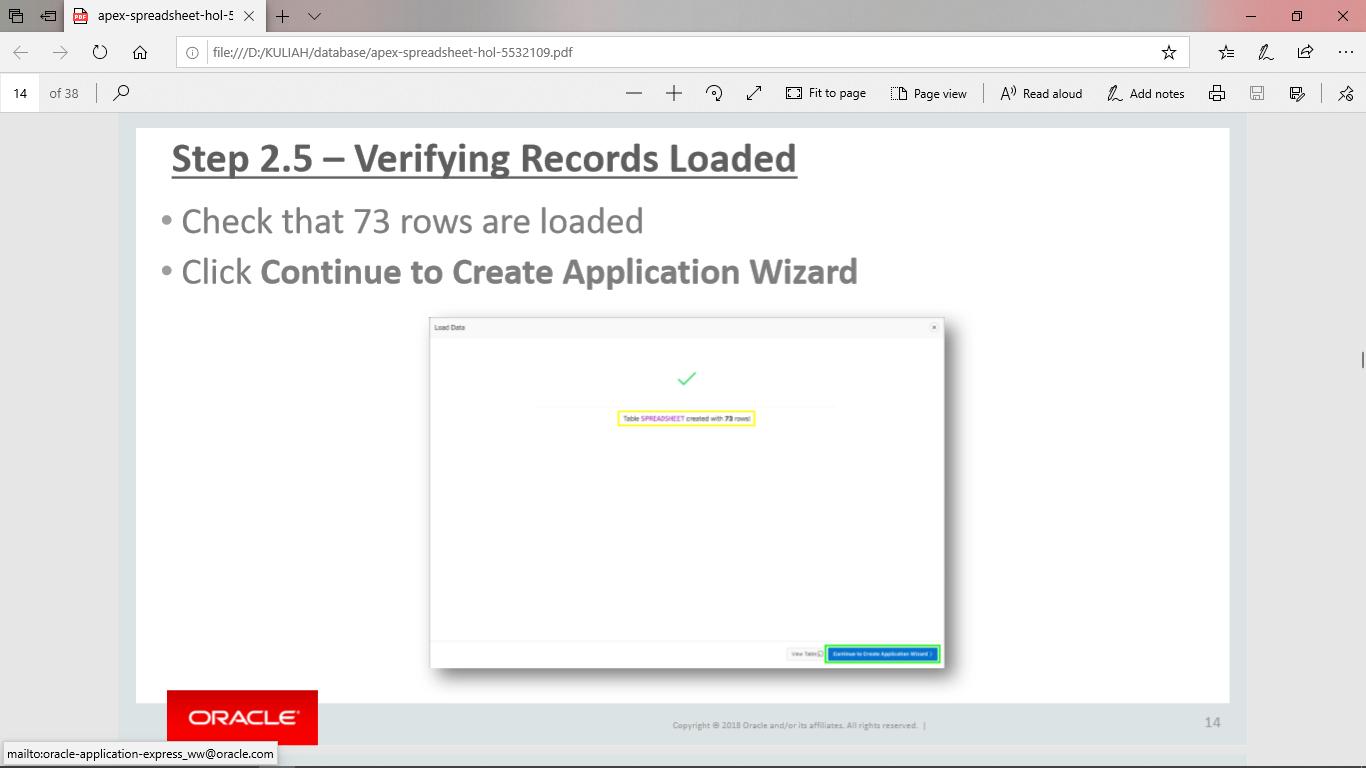
\includegraphics[scale=0.3]{figures/pic(8).png}
    \caption{\textit{Oracle Apex Load Data.}}
        \end{center}
\label{gambar}
\end{figure}

\begin{figure}
\item[16] Beri nama lalu ke features dan check all.

    \begin{center}
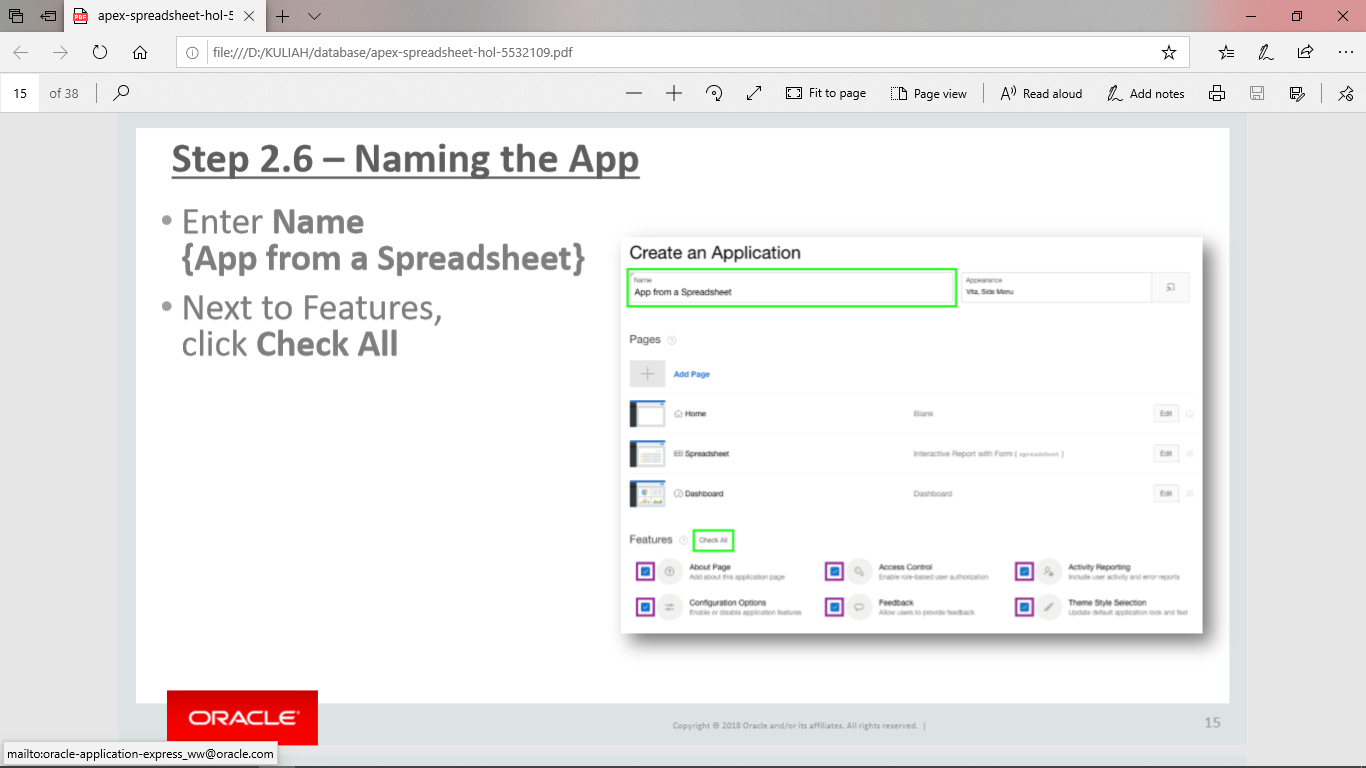
\includegraphics[scale=0.3]{figures/pic(9).png}
    \caption{\textit{naming the app.}}
        \end{center}
\label{gambar}
\end{figure}

\begin{figure}
\item[17] Buat aplikasi baru

    \begin{center}
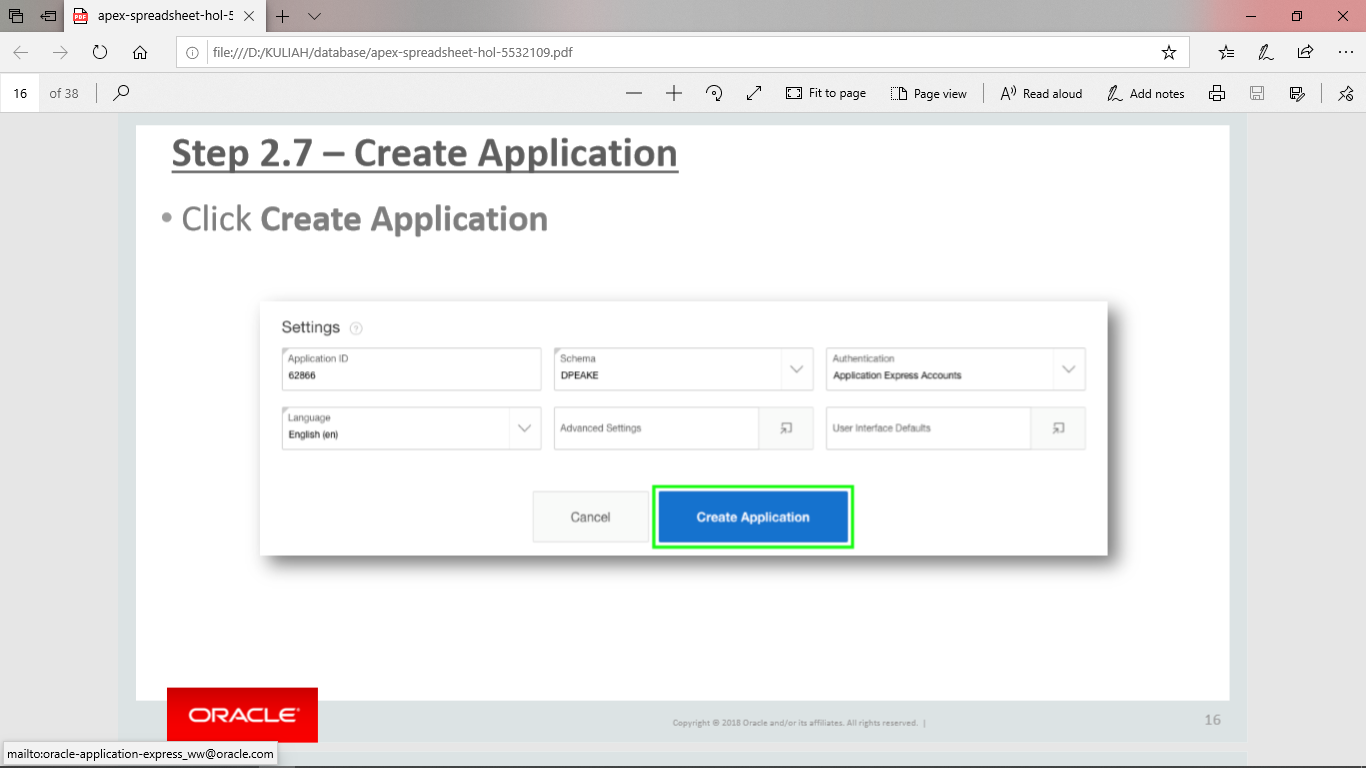
\includegraphics[scale=0.3]{figures/pic(10).png}
    \caption{\textit{Create application.}}
        \end{center}
\label{gambar}
\end{figure}

\begin{figure}
\item[18] Aplikasi baru tersebut sudah ditampilkan di halaman design lalu jalankan aplikasi.

    \begin{center}
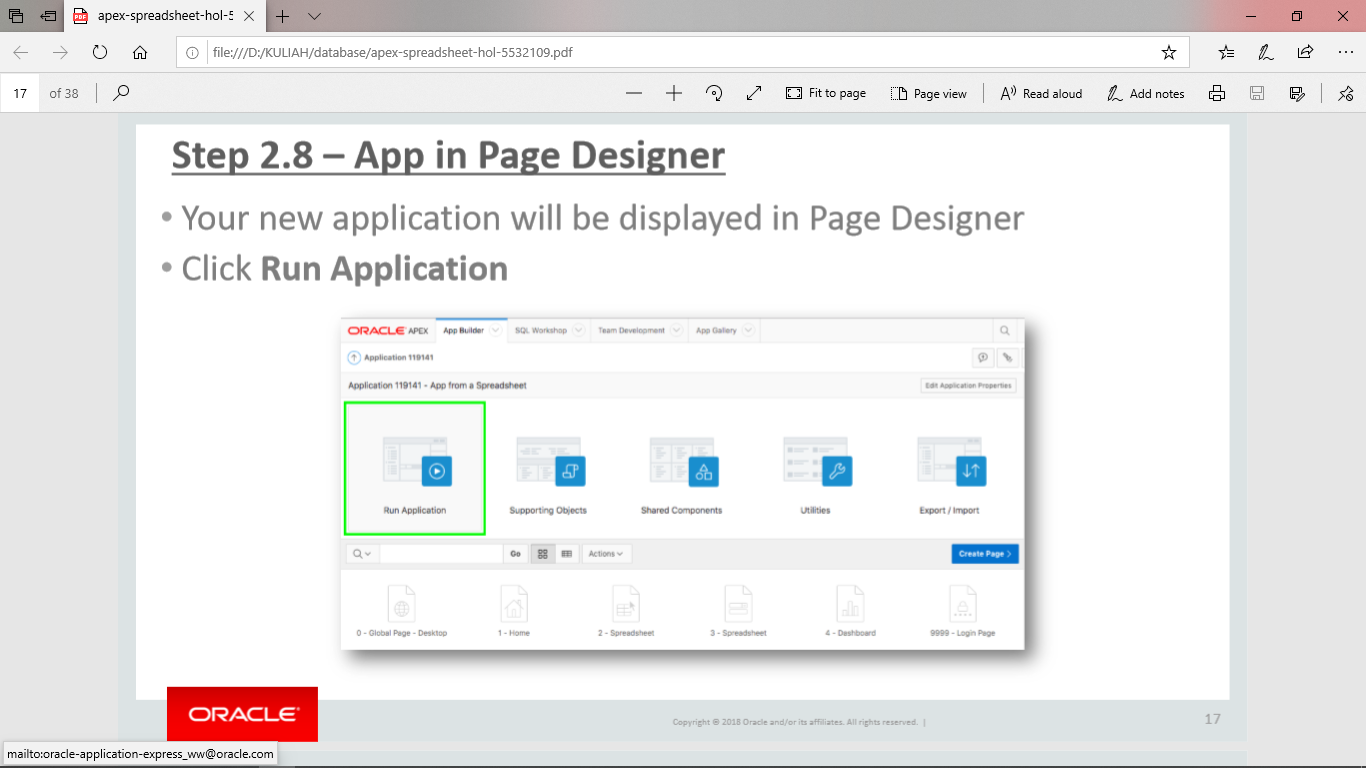
\includegraphics[scale=0.3]{figures/pic(11).png}
    \caption{\textit{app in page designer.}}
        \end{center}
\label{gambar}
\end{figure}


\begin{figure}
\item[19] Masukkan kredensial pengguna anda dan mulai jalankan dengan aplikasi baru.

    \begin{center}
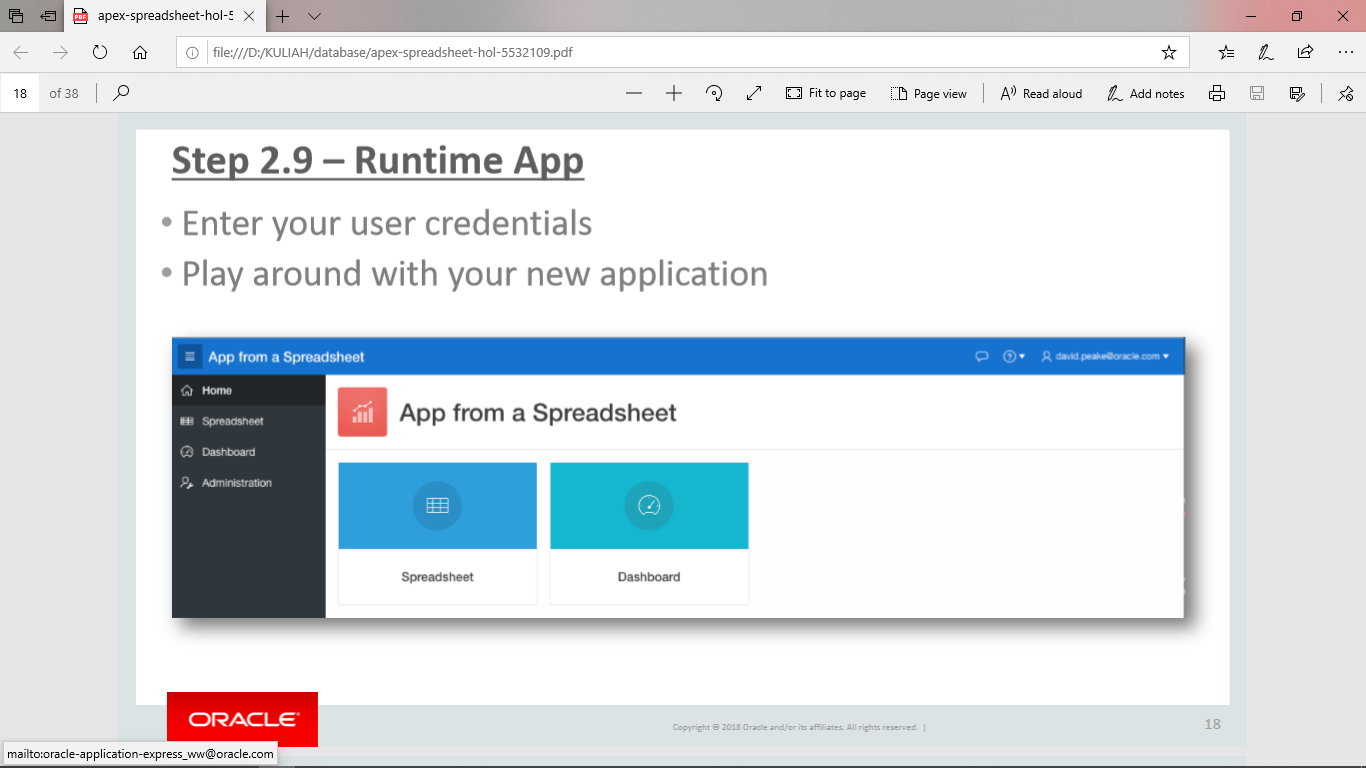
\includegraphics[scale=0.3]{figures/pic(12).png}
    \caption{\textit{run time app.}}
        \end{center}
\label{gambar}
\end{figure}


\end{enumerate}
